\section{Formalising requirements}
\subsection{}

\begin{frame}
\frametitleTC{A time-domain viewpoint}
\framesubtitleTC{}
\myPause
 \begin{itemize}[<+-| alert@+>]
 \item Requirements are expressed in the time domain very naturally.
 \item Suppose to apply a step variation to the set point $w(k)$, and consider four possible\\
       responses of the controlled variable $y(k)$ --- points are joined with segments\\
       to improve readability:
       \begin{center}
        \vspace{2mm}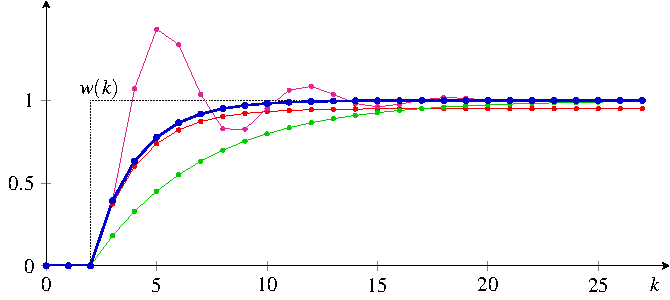
\includegraphics[width=0.60\columnwidth]{./Unit-04/img/StepRespForRequirements.pdf}
       \end{center}
 \end{itemize}
\end{frame}

\begin{frame}
\frametitleTC{A time-domain viewpoint}
\framesubtitleTC{}
\myPause
 \begin{center}
  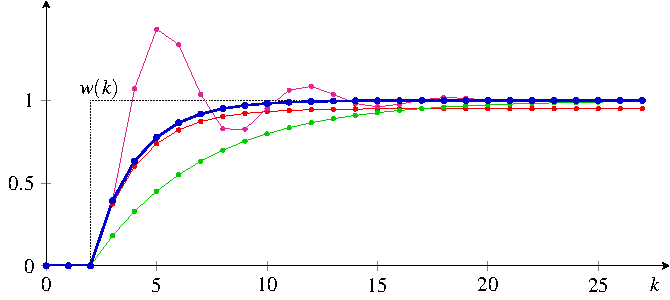
\includegraphics[width=0.40\columnwidth]{./Unit-04/img/StepRespForRequirements.pdf}
 \end{center}\myPause
 \begin{itemize}[<+-| alert@+>]
 \item The ``control quality'' (for the moment, in the most intuitive sense)\\
       is different:
       \begin{itemize}[<+-| alert@+>]
       \item \textcolor{blue!80!black}{blue} -- good;
       \item \textcolor{red!95!black}{red} -- does not reach the new desired value exactly;
       \item \textcolor{green!80!black}{green} -- too slow;
       \item \textcolor{magenta!95!black}{magenta} -- oscillatory.
       \end{itemize}
 \end{itemize}
\end{frame}

\begin{frame}
\frametitleTC{A time-domain viewpoint}
\framesubtitleTC{}
\myPause
 \begin{itemize}[<+-| alert@+>]
 \item Indeed, many requirements are straightforwardly expressed by stating e.g. how the response
       of the controlled variable to a certain variation of the set point has to look.
 \item For example, one may require that
       \begin{itemize}[<+-| alert@+>]
       \item[] when $w(k)$ undergoes a step variation
       \item[] $y(k)$ has to enter a $\mp$5\% band around it in maximum 5 steps
       \item[] and then never exit that band,
       \item[] also never reaching a value more than 10\% above the new set point,
       \item[] and with a one-step variation not greater than half of the total one,
       \end{itemize}
 \item[] or express analogous desires.
 \end{itemize}
\end{frame}

\begin{frame}
\frametitleTC{A time-domain viewpoint}
\framesubtitleTC{}
\myPause
 \begin{itemize}[<+-| alert@+>]
 \item A quite articulated example to illustrate the idea is shown below: the response has to lie
       entirely within the evidenced area.
       \begin{center}
        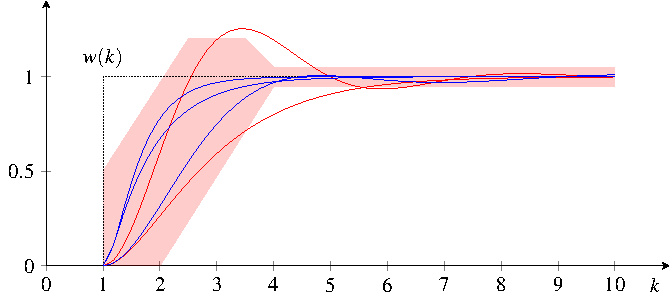
\includegraphics[width=0.60\columnwidth]{./Unit-04/img/StepRespWithConstraints-SP.pdf}
       \end{center}
 \item Blue responses are acceptable, red ones are not.
 \end{itemize}
\end{frame}


\begin{frame}
\frametitleTC{A time-domain viewpoint}
\framesubtitleTC{}
\myPause
 \begin{itemize}[<+-| alert@+>]
 \item The key idea we are soon introducing is that prescribing a certain aspect for the response
       of $y(k)$ to $w(k)$, in fact means prescribing characteristics of the transfer function
       from the former to the latter (as already anticipated).
 \item The same idea can be applied to the responses of $y(k)$ to disturbances, if the issue is to
       reject them.
 \item \vspace{3mm}This is not the only way to set requirements, but here we stick to this one.
 \item In the following we shall see how the idea above leads to synthesising\\
       a suitable controller --- and the PID structure will come into play\\
       \TC{with consciousness of the reasons for its wide applicability}.
 \item \vfill But prior to this, also to understand what a reasonable ``desired $y/w$\\
       transfer function'' can look like, we need to analyse the control loop\\
       formally.
 \end{itemize}
\end{frame}
